%%%%%%%%%%%%%%%%%%%%%%%%%%%%%%%%%%%%%%%%%%%%%%%%%%%%%%%
%% Bachelor's & Master's Thesis Template             %%
%% Copyleft by Artur M. Brodzki & Piotr Woźniak      %%
%% Faculty of Electronics and Information Technology %%
%% Warsaw University of Technology, 2019-2020        %%
%%%%%%%%%%%%%%%%%%%%%%%%%%%%%%%%%%%%%%%%%%%%%%%%%%%%%%%

\documentclass[
    left=2.5cm,         % Sadly, generic margin parameter
    right=2.5cm,        % doesnt't work, as it is
    top=2.5cm,          % superseded by more specific
    bottom=3cm,         % left...bottom parameters.
    bindingoffset=6mm,  % Optional binding offset.
    nohyphenation=false % You may turn off hyphenation, if don't like.
]{eiti/eiti-thesis}

\langpol % Dla języka angielskiego mamy \langeng
\graphicspath{{img/}}             % Katalog z obrazkami.
\addbibresource{bibliografia.bib} % Plik .bib z bibliografią
\usepackage{subfig}

\begin{document}

%--------------------------------------
% Strona tytułowa
%--------------------------------------
\MasterThesis % Dla pracy inżynierskiej mamy \EngineerThesis
\instytut{Informatyki}
\kierunek{Informatyka}
\specjalnosc{Inzynieria systemow informatycznych}
\title{
    Aplikacja internetowa do rozliczania\\ wspólnych wydatków
}
\engtitle{ % Tytuł po angielsku do angielskiego streszczenia
    Unnecessarily long and complicated thesis' title \\
    difficult to read, understand and pronounce
}
\author{Jarosław Glegoła}
\album{293092}
\promotor{dr inż. Roman Podraza}
\date{\the\year}
\maketitle

%--------------------------------------
% Streszczenie po polsku
%--------------------------------------
\cleardoublepage % Zaczynamy od nieparzystej strony
\streszczenie \lipsum[1-3]
\slowakluczowe XXX, XXX, XXX

%--------------------------------------
% Streszczenie po angielsku
%--------------------------------------
\newpage
\abstract \kant[1-3]
\keywords XXX, XXX, XXX

%--------------------------------------
% Oświadczenie o autorstwie
%--------------------------------------
\cleardoublepage  % Zaczynamy od nieparzystej strony
\pagestyle{plain}
\makeauthorship

%--------------------------------------
% Spis treści
%--------------------------------------
\cleardoublepage % Zaczynamy od nieparzystej strony
\tableofcontents

%--------------------------------------
% Rozdziały
%--------------------------------------
\cleardoublepage % Zaczynamy od nieparzystej strony
\pagestyle{headings}

\newpage % Rozdziały zaczynamy od nowej strony.
\section{Wprowadzenie}

Zdarza się w naszym życiu, że razem z innymi osobami kupujemy rzeczy, za które płaci tylko jedna osoba. W takiej sytuacji dosyć uciążliwe może być proszenie innych osób o zwrot kwoty, obliczanie owej kwoty, którą należy zwrócić płatnikowi, oraz śledzenie wszystkich płatności i wydatków, w których uczestniczyliśmy. W takiej sytuacji dobrym pomysłem byłoby użycie aplikacji lub programu komputerowego, który pomagałby nam w śledzeniu takich elementów naszego życia. W ramach tej pracy została utworzona właśnie taka aplikacja i została nazwana Aprint.

\subsection{Opis przypadku biznesowego}
\subsubsection{Opis hipotetycznej sytuacji}

Aby bardziej zilustrować przypadek biznesowy, możemy wyobrazić sobie sytuację, w której dwóch współlokatorów (nazwijmy ich Rafał i Kacper) mieszka w jednym mieszkaniu i obydwaj wydają pieniądze na rzeczy potrzebne na utrzymanie całego mieszkania. Pewnego dnia Rafał kupuje środki czystości. Jak możemy się domyślić, środki czystości będą używane przez Kacpra i Rafała, natomiast w tej hipotetycznej sytuacji tylko Rafał zapłacił w całości za owe produkty. Z tego powodu Kacper jest winny części kwoty Rafałowi. Obydwaj używając aplikacji, mogą w prosty sposób rozliczyć się z tego wydatku.

\subsubsection{Użycie aplikacji}

Na samym początku Rafał musi utworzyć obiekt wydatku na stronie internetowej, używając do tego dedykowanego formularza, wypełniając takie informacje jak nazwa wydatku, jego opis, datę kiedy ten wydatek został stworzony oraz osoby, które razem z nim z brali udział w wydatku (w tym wydatku tylko Kacpra).

Gdy wydatek zostanie utworzony, Kacper będzie mógł potwierdzić lub odrzucić udział w owej transakcji. Będzie mógł to zrobić na dedykowanym ekranie płatności, na którym będą odpowiednie przyciski oraz informacje dotyczące płatności, takie jak opis, data utworzenia wydatku itp. Jeżeli Kacper potwierdzi to, że brał udział w tym wydatku, będzie mógł nacisnąć przycisk \emph{potwierdzam płatność}, a jeżeli się z tym nie zgadza, naciśnie przycisk \emph{odrzucam płatność}.

Gdy wszyscy uczestnicy wydatku (w tym przypadku tylko Kacper) potwierdzi lub odrzuci udział, inicjator wydatku będzie mógł zatwierdzić uczestników, czyli kliknąć przycisk na ekranie wydatku o treści "potwierdzam użytkowników". To potwierdzenie nie mogło zostać zaimplementowane automatycznie, ponieważ inicjator wydatku może nie zgodzić się z uczestnikami i w takim wydatku może z nimi porozmawiać lub wyjaśnić niespójności.

Następnym krokiem tego scenariusza jest już sama akcja zapłaty za wydatek. Uczestnik wydatku Kacper może przejść na ekran płatności, na którym będzie już obliczona kwota, którą Kacper musi zapłacić Rafałowi. Po płatności ze strony Kacpra będzie mógł on kliknąć przycisk "potwierdzam płatność" i uregulować w ten sposób należność.

Ostatnim elementem scenariusza jest zakończenie wydatku przez inicjatora wtedy, kiedy wszyscy uczestnicy uregulują swoje płatności. Będzie on mógł to zrobić na ekranie wydatku po kliknięciu w przycisk zakończ wydatek.

\subsection{Układ pracy}
Praca jest podzielona na 4 rozdziały, gdzie w pierwszym zostaną opisane wymagania, jakie aplikacja do zarządzania wspólnymi wydatkami powinna spełniać. W drugim rozdziale zostaną opisane użyte technologie i podejścia, które zostały użyte podczas pisania aplikacji. W kolejnym rozdziale zostaną opisane różne sposoby automatycznego testowania aplikacji internetowej. W ostatnim rozdziale zostanie przedstawiony wygląd i poszczególne ekrany aplikacji.


         % Wygodnie jest trzymać każdy rozdział w osobnym pliku.
\newpage % Rozdziały zaczynamy od nowej strony.

\section{Specyfikacja wymagań}
\subsection{Słownik pojęć}
\begin{description}
  \item[Użytkownik] \hfill \\ Osoba, która złożyła konto w mojej aplikacji, posiadająca unikalny e-mail oraz inne dane osobowe.
  \item[Wydarzenie] \hfill \\ Obiekt reprezentujący wydarzenie, do którego moją dołączać użytkownicy aplikacji. Wydarzenie posiada nazwę, godzinę rozpoczęcia i zakończenia, listę uczestników, opis, współrzędne wybrane geograficzne miejsca, w którym wydarzenie będzie miało miejsce oraz listę wydatków.
  \item[Grupa] \hfill \\ Obiekt reprezentujący grupę użytkowników, która by chciała rozliczać wspólne wydatki, bez ustalonych ram czasowych lub ustalonego miejsca. Posiada nazwę, opis, listę uczestników oraz listę wydatków.
  \item[Wydatek] \hfill \\ Obiekt reprezentujący pojedynczy wydatek utworzony w prawdziwym życiu przez użytkownika, który zawiera nazwę, opis, kwotę uiszczoną za daną transakcję, datę płatności oraz osoby, które według osoby tworzącej wydatek wspólnie brały udział w wydatku.
  \item[Uczestnik wydatku] \hfill \\ Użytkownik, który jest na liście uczestników w danym wydatku i posiada swoją własną płatność należącą do tegoż wydatku.
  \item[Płatność] \hfill \\ Część wydatku, która posiada informacje dotyczące każdego z uczestników wydatku. Płatność może znajdować się w stanie:
    \begin{itemize}
    \item oczekującym - użytkownik został zaproszony do wydatku i może on potwierdzić lub odrzucić w niej udział 
    \item zaakceptowanym - użytkownik potwierdził udział w wydatku i zgodził się na zapłacenie części kwoty
    \item odrzuconym - użytkownik nie zgodził się na udział w wydatku
    \item opłaconym - użytkownik po zaakceptowaniu płatności opłacił swoją część
    \item todo - reszta stanów
  \end{itemize}
\item[Zaproszenie] \hfill \\ W trakcie zakładania grupy lub wydarzenia użytkownik ma możliwość wskazania uczestników. Po utworzeniu obiektu każdemu wybranemu użytkownikowi wysyłane jest zaproszenie, które wybrany użytkownik może zaakceptować (potwierdzić udział w wydarzeniu lub grupie) lub je odrzucić.
\item[Znajomy] \hfill \\ Użytkownik, który został zaproszony do listy znajomych. Tylko znajomi mogą być zapraszani do grup wydarzeń i wydatków.
\end{description}


\subsection{Wymagania funkcjonalne}
\begin{description}
  \item[WF1.] \hfill \\ Użytkownik może założyć konto w aplikacji podając adres e-mail, hasło oraz imię i nazwisko.
  \item[WF2.] \hfill \\ Użytkownik może zalogować się do mojej aplikacji z użyciem adresu e-mail i hasła podanego przy rejestracji.
  \item[WF3.] \hfill \\ Użytkownik może dodawać innych użytkowników do znajomych.
  \item[WF4.] \hfill \\ Użytkownik może zakładać wydatki podając takie informacje jak:
    \begin{itemize}
      \item nazwa
      \item rodzaj wydatku: 
        \begin{itemize}
          \item wydatek w ramach wydarzenia
          \item wydatek w ramach grupy
          \item wydatek bez grupy
        \end{itemize}
      \item uczestników wydatku
      \item kwoty wydanej w ramach wydatku
      \item kwoty która przypada na każdego użytkownika
      \item datę opłacenia wydatku
      \item opis
    \end{itemize}
  \item[WF5.] \hfill \\ Użytkownik może zarządzać stanem swoich płatności. Może je: akceptować, odrzucać i potwierdzać płatność.
  \item[WF6.] \hfill \\ Użytkownik może zarządzać stanem swoich wydarzeń i grup. Może dodawać nowych uczestników, usuwać uczestników, zmieniać datę wydarzenia, opis, miejsce.
  \item[WF7.] \hfill \\ Użytkownik może zarządzać stanem swoich wydatków. Może zmieniać ich opis datę, nazwę i kwotę.
  \item[WF8.] \hfill \\ Użytkownik dostaje powiadomienia za każdym razem gdy:
    \begin{itemize}
      \item dostaje nowe zaproszenie do grupy lub wydarzenia
      \item zmienia się stan wydatku
      \item zmienia się stan płatności
    \end{itemize}
  \item[WF9.] \hfill \\ Użytkownik może zarządzać zaproszeniami, czyli przeglądać listę zaproszeń, akceptować lub odrzucać poszczególne zaproszenia
  \item[WF10.] \hfill \\ Użytkownik posiada statystyki dotyczące swoich wydatków, czyli jaką kwotę powinien oddać innym użytkownikom oraz ile inni użytkownicy powinni oddać użytkownikowi oddać. Statystyki te są dostępne per osoba oraz podsumowujące wszystkie wydatki użytkownika ze wszystkimi innymi użytkownikami.
\end{description}

\subsection{Wymagania funkcjonalne}
\begin{description}
  \item[WN1.] \hfill \\ Aplikacja działa na najnowszych przeglądarkach: Chrome, Firefox oraz Edge.
  \item[WN2.] \hfill \\ Aplikacja jest renderowana po stronie klienta z wykorzystaniem reaktywnej biblioteki Javascript.
  \item[WN3.] \hfill \\ Komunikacja aplikacji z serwerem odbywa się poprzez bezpieczne połączenie https.
  \item[WN4.] \hfill \\ Aplikacja komunikuje się z serwerem zgodnie ze specyfikacją GraphQL.
  \item[WN5.] \hfill \\ Aplikacja poprawnie wyświetla się na rozdzielczościach z przedziału 360px - 1600px.
  \item[WN5.] \hfill \\ Rozmiar skryptów klienckich nie powinien przekraczać 2MB.
  \item[WN6.] \hfill \\ Autoryzacja odbywa się przy użyciu tokenów JWT.
\end{description}
% // todo reguły biznesowe może
         % Wygodnie jest trzymać każdy rozdział w osobnym pliku.
\newpage
\section{Użyte technologie}
Aplikacja jest podzielona na dwie główne części: część serwerową i część kliencką. Obie części są niezbędne do działania mojego systemu.
Część serwerowa jest odpowiedzialna za przetwarzanie danych, operacje na bazie danych, zarządzanie zapytaniami pochodzącymi z aplikacji klienckiej oraz zapewnieniem bezpieczeństwa użytkownika. Aplikacja została napisana w języku Kotlin z użyciem bardzo popularnej biblioteki Spring. Dodatkowo została także użyta biblioteka graphql-kotlin, która udostępnia przejrzysty interfejs umożliwiający w prosty sposób tworzenie serwisu, z którym można komunikować się zgodnie z specyfikacją GraphQL.


Część kliencka jest odpowiedzialna za wyświetlanie aktualnych danych użytkownikowi, udostępnia przejrzysty interfejs, dzięki któremu użytkownik może zarządzać swoim kontem oraz powiązanymi z nim obiektami. 

// todo rysunek obrazujący połączenie i rozmieszczenie elementów systemu.

\subsection{Warstwa serwera}
Aktualnie istnieje wiele różnych podejść do pisania aplikacji serwerowych, które mają ułatwiać pisanie, rozwijanie i utrzymywanie większych systemów. Jednym z takich podejść jest Architektura Heksagonalna, której użyłem do stworzenia mojej aplikacji.
\subsubsection{Architektura}
Podczas tworzenia mojej aplikacji serwerowej kierowałem się podejściem zwanym Architekturą Heksagonalną (lub Architektura Portów i Adapterów).
Architektura Heksagonalna została udokumentowana przez Alistaira Cockburna w 2005. Aktualnie jest bardzo popularnym podejściem do tworzenia mikroserwisów, ponieważ umożliwia ona w łatwy sposób rozbudowywanie aktualnego rozwiązania jak i wprowadzanie zmian wynikających ze zmian w architekturze systemu.
Główne cechy Heksagonalnej Architektury to:
\begin{itemize}
  \item oddzielenie strony klienckiej, logiki biznesowej oraz strony serwerowej
  \item podział komponentów serwera na tzw. porty i adaptery
\end{itemize}
Główne idee kierujące tą architekturą to:
\begin{description}
  \item[Logika biznesowa] \hfill \\ Główną i najważniejszą częścią naszego systemu jest logika biznesowa. Reguły biznesowe i zasady nimi rządzące nie powinny być w żaden sposób mocno bazować na innych komponentach systemu. Powinny zawierać tylko i wyłącznie elementy związane z logiką naszego systemu, a elementy infrastruktury (jak np. bazy danych, zewnętrzne serwisy) powinny być zależne od komponentu logiki biznesowej. Odizolowanie tej części ma kilka zalet:
\begin{itemize}
  \item Logika biznesowa jest bardzo łatwo testowalna jednostkowo. Jako że testy nie bazują na zewnętrznych narzędziach lub serwisach, tylko na ich interfejsach, możliwe jest w łatwy sposób pisanie testów symulujących działanie zewnętrznych narzędzi. Rzeczy takie jak komunikacja z bazą danych lub operacje na żądaniach klienckich nie są wymagane do pisania takich testów, więc pisze się je szybko i są one bardzo czytelne.
  \item Kod logiki jest czytelny i prosty, ponieważ nie powinien on zawierać elementów infrastruktury. Z tego powodu nawet osoby, które znają zasady biznesowe naszego sytemu, ale nie są osobami technicznymi, mogą być w stanie zrozumieć fragmenty kodu domenowego.
\begin{addmargin}[6mm]{0mm}
\begin{lstlisting}[
    numbers=left,
    firstnumber=1,
    caption={Przykład kodu domenowego aplikacji w języku Koltin},
    aboveskip=10pt
]
fun deleteParty(id: Long, currentUserId: Long): Party? {
        val party = partyRepository.getTopById(id)

        if (party?.owner?.id != currentUserId) {
            throw UnauthorisedException()
        }

        partyRepository.removeParty(id)

        return party
}
\end{lstlisting}
\end{addmargin}
  Jak można zauważyć w powyższym kodzie nie ma odwołań do bazy danych ani do żądania, tylko są jedynie zasady dotyczące działania systemu, czyli tylko założyciel grupy ma możliwość usunięcia danej grupy.
  \item Bardzo łatwo można wymieniać części systemu nie związane z logiką biznesową np. bazy danych, zewnętrzne serwisy. Szczególnie w dobie mikroserwisów, wymiana zewnętrzych serwisów jest rzeczą wcale rzadką, więc gdy chcemy zmienić np. API do zewnętrznej części systemu to jeżeli będziemy się trzymać kontraktu na którym bazuje nasza logika biznesowa, to nie będą potrzebne zmiany w głównej części naszej aplikacji.
\end{itemize}


\item[Adaptery] \hfill \\ Adaptery są elementami które "wychodzą na świat", czyli są one odpowiedzialne za komunikację z zewnętrznymi serwisami. Adapterem jest np. część systemu odpowiadająca za zdefiniowanie kwerend i mutacji GraphQL'owych, komponenty komunikujące się z zewnętrznymi serwisami lub części komunikujące się z bazą danych. Adaptery są zależne od części domenowej aplikacji tj. są zależne od modeli domenowych naszej aplikacji. Komponenty logiki biznesowej używają adapterów z użyciem własnych modeli domenowych, a żeby adaptery mogły korzystać z tych modeli, muszą one je przekonwertować na swoją reprezentację. Przykładowo powiedzmy, że mamy model biznesowy \emph{Grupa}, którą możemy zaprezentować w klasie Kotlinowej tak:


\begin{addmargin}[6mm]{0mm}
\begin{lstlisting}[
    numbers=left,
    firstnumber=1,
    caption={Klasa \emph{Grupa} w domenowej reprezentacji modelu},
    aboveskip=10pt
]
data class Grupa(
    val id: Long?,
    val imie: String?,
)
\end{lstlisting}
\end{addmargin}

a model adapteru komunikującego się z bazą danych tak:
\begin{addmargin}[6mm]{0mm}
\begin{lstlisting}[
    numbers=left,
    firstnumber=1,
    caption={Klasa \emph{Grupa} w domenowej reprezentacji modelu},
    aboveskip=10pt
]
data class GrupaAdapter(
    val id: Long?,
    val imie: String?,
    val rowId: String?,
)
\end{lstlisting}
\end{addmargin}
Te dwa modele różnią się tym, że adapterowy model posiada dodatkowy atrybut związany z bazą danych \emph{rowId}. Model domenowy nie potrzebuje tego atrybutu, a nawet nie powinien wiedzieć, że taki atrybut istnieje. W takim wypadku, jeżeli te dwa modele są różne, przy komunikacji pomiędzy częścią domenową i adapterową musi nastąpić translacja modeli. Wcześniej napisałem, że część domenowa nie powinna być zależna od innych części systemu, dlatego tę odpowiedzialność wykonują adaptery. Komponent domenowy, w naszym przykładzie może komunikować z adapterem przez taki interfejs:
\begin{addmargin}[6mm]{0mm}
\begin{lstlisting}[
    label={lst:AdapterBazyDanychPort},
    numbers=left,
    firstnumber=1,
    caption={Interfejs domenowy adaptera bazy danych},
    aboveskip=10pt
]
interface AdapterBazyDanych {
    fun zapiszNowaGrupa(grupa: Grupa): Grupa
}
\end{lstlisting}
\end{addmargin}
Jak widzimy komponent domenowy nie posługuje się nigdy klasą adaptera, tylko adapter który implementuje ten interfejs musi przeprowadzić konwersję argumentu \emph{grupa} przy wywoływaniu funkcji oraz przy zwracaniu wartości z tej funkcji.

\item[Porty] \hfill \\ Porty są zwykłym kontraktem pomiędzy komponentem logiki biznesowej, a adapterami. Porty posiadają logiki tylko służą do oddzielenia odpowiedzialności komponentów naszego systemu. Przykładem portu może być wcześniej podany przykład interfejsu \emph{AdapterBazyDanych} w listingu~\ref{lst:AdapterBazyDanychPort}. 

\end{description}
Moja aplikacja zawiera obiektów reprezentujących cały system. Są to:
\begin{itemize}
  \item wydatek
  \item powiadomienie
  \item grupa
  \item zaproszenie
  \item płatność
  \item użytkownik
\end{itemize}
, a moja aplikacja jest podzielona na trzy części:
\begin{itemize}
  \item adapter klienta - adapter zajmujący się definiowaniem i obsługą zapytań klienta
  \item część domenowa - główna część mojej aplikacji zajmująca się definiowaniem reguł biznesowych
  \item adapter bazodanowy - zajmujący się obsługą bazy danych
\end{itemize}
Dla każdego obiektu jest stworzony osobny komponent w każdej z części. Jeżeli weźmiemy pod uwagę np. obiekt grupa to:
// todo tu mogą być fragmenty kodu kontrollera serwisu i repozytorium
\begin{enumerate}
  \item Adapter klienta będzie nazywał się \emph{GrupaResolver} i będzie definiował wszystkie dostępne kwerendy i mutacje dla grupy.
    % \begin{addmargin}[6mm]{0mm}
    % \begin{lstlisting}[
    %     numbers=left,
    %     firstnumber=1,
    %     caption={Interfejs domenowy adaptera bazy danych},
    %     aboveskip=10pt
    % ]
    % class GrupaQuery(private val grupaSerwis: GrupaSerwis): Query {
    %   fun pobierzWszystkieGrupy(uzytkownikId: String):
    %     List<GrupaDTO> =
    %           grupaSerwis.pobierzWszystkieGrupy(
    %             uzytkownikId
    %           ).map { it.doDTO() }

    %   fun pobierzGrupe(grupaId: String): GrupaDTO? = 
    %     grupaSerwis.pobierzGrupe(grupaId)?.doDTO()
    % }
    % \end{lstlisting}
    % \end{addmargin}
  \item Logika domenowa dla grupy która będzie się nazywała \emph{GrupaSerwis} gdzie będzie znajdowała się logika związana z obsługą grupy.
  \item Adapter bazodanowy który będzie nazywał się \emph{GrupaPersistentRepository} gdzie będzie znajdowała się komunikacja z bazą danych.
    
\end{enumerate}

\subsubsection{Główne użyte technologie}
Do stworzenia aplikacji serwerowej użyłem następujących technologii:

\begin{description}
  \item[Kotlin] \hfill \\ Głównym językiem programowania jakiego użyłem do napisania aplikacji serwerowej jest Kotlin. Kotlin jest zorientowanym obiektowo, statycznie typowanym językiem programowania. Kotlin jest oparty na JVM, więc technologie i biblioteki, które zostały stworzone w języku Java, mogą być także używane w języku Kotlin. 
  \item[Spring] \hfill \\ Spring jest wolnoźródłowym frameworkiem do budowania aplikacji serwerowych w językach opartych na JVM. Posiada on dużą ilość potrzebnych przy tworzeniu aplikacji serwerowych funkcjonalności. 

    Podstawową funkcją udostępnianą przez Spring Framework jest kontener do wstrzykiwania zależności. Spring umożliwia nam tworzenie pojedynczych komponentów, które później mogą być \emph{wstrzyknięte} jako zależności do innych komponentów. Jeżeli komponent \emph{A} zależy od komponentu \emph{B}, czyli \emph{A} używa \emph{B}, aby móc zrealizować swoją własną funkcję, \emph{A} nie musi sam tworzyć instancji \emph{B} tylko może np. dać znać Springowi, że jest zależny od komponentu \emph{B} poprzez umieszczenie \emph{B} np. jako parametr w konstruktorze. W takiej sytuacji gdy obiekt \emph{A} będzie tworzony, kontener będzie automatycznie wywoływał konstruktor \emph{A} z odpowiednimi parametrami.

    Dodatkowo Spring posiada bardzo dużo innych narzędzi, dzięki którym można budować duże serwisy, takie jak:
    \begin{enumerate}
      \item \textbf{Spring Boot} - narzędzie pozwalające w bardzo szybki sposób skonfigurować serwer aplikacji wraz z wszystkimi potrzebnymi elementami potrzebnymi do działania takiego serwisu np. autoryzacji lub komunikację z bazą danych. Dzięki niemu możemy otrzymać podstawową konfigurację do modułów wymienionych poniżej, czyli np. Spring Security lub Spring Data JPA
      \item \textbf{Spring Security} - moduł, która odpowiada za bezpieczeństwo naszej aplikacji. Domyślnie po zainstalowaniu tego modułu mamy dostęp do narzędzi, które pozwalają nam np. autoryzować użytkownika, konfigurować CORS, blokować niektóre endpointy itp.
      \item \textbf{Spring Data JPA} - JPA jest to standard ORM dla języka Java. Dzięki JPA mamy mechanizmy, które pozwalają nam zarządzać bazą danych z poziomu kodu programu, bez użycia SQL. Przy takim podejściu klasy w języku Kotlin mogą być mapowane na elementy tabel w bazie danych przy zapisie lub ich edycji. Dodatkowo przy odczycie tych danych elementy tabel w bazie danych mogą być mapowane z powrotem na klasy Kotlinowe. Dzięki temu w łatwy sposób możemy zapewnić spójność pomiędzy modelami bazodanowymi a modelami w Kotlinie. Jako że JPA jest tylko standardem, aby móc robić takie rzeczy w Springu potrzebujemy narzędzia, które będzie ten standard implementować. Jednym z takich narzędzi, które wybrałem jest biblioteka Hibernate, która jest domyślnie wspierana przez framework Spring i może być łatwo skonfigurowana z użyciem Spring Boot.
    \end{enumerate}

  \item[PostgreSQL] \hfill \\ PostgreSQL jest jedną z kilku najpopularniejszych wolnoźródłowych baz danych. Jest to relacyjna baza danych, która jest wspierana przez framework Spring. Baza danych jest obsługiwana z języka Kotlin i przechowywane są w niej wszystkie dane użytkownika.
  \item[GraphQL-Kotlin] \hfill \\ Biblioteka GraphQL-Kotlin jest zbudowana na innej bibliotece `graphql-java`, która ułatwia tworzenie aplikacji serwerowych udostępniających interfejs poprzez standard graphql. Udostępnia ona domyślnie funkcjonalność odbierania i parsowania zapytań graphqlowych, posiada funkcje pozwalające obsługiwać błędy w zapytaniach oraz tworzenia odpowiedzi do klienta zgodnie ze owym standardem.
\end{description}


\subsection{Warstwa komunikacji - GraphQL}
W moim projekcie, zamiast użycia bardzo popularnego standardu do komunikacji między klientem a serwerem jakim jest REST, postanowiłem użyć standardu GraphQL.

GraphQL jest specyfikacją utworzoną przez Facebooka, który opisuje sposób, w jaki dwie jednostki mogą się ze sobą komunikować. Jest to językiem zapytań, który może zostać użyty przez klienta, aby otrzymać dane, które wskaże w zapytaniu. W przeciwieństwie do REST, gdzie odpowiedzi serwera dla każdego endpointu są ustalone z góry. GraphQL nie jest protokołem sieciowym, a tylko kontraktem między jednostkami.

Serwer udostępniając interfejs GraphQL, definiuje tzw. schemat GraphQL, czyli statycznie i mocno typowany opis wszystkich możliwych operacji oraz typów dostępnych klientowi używającego danego interfejsu. 

\begin{addmargin}[6mm]{0mm}
\begin{lstlisting}[
    numbers=none,
    firstnumber=1,
    label={lst:graphqlSchema}
    caption={Przykład schematu GraphQL},
    aboveskip=10pt
]
type Grupa {
  id: String!;
  nazwa: String!;
  uczestnicy: [Uzytkownik!];
  opis: String!;
}
type Uzytkownik {
  id: String!;
  nazwisko String!;
}
type Powiadomienie {
  id: String!;
  tresc: String!;
}
type Query {
  pobierzGrupe(idGrupy: String!): Grupa
}
type Mutation {
  zapiszNowaGrupa(grupa: Grupa!): Boolean
}
type Subscription {
  pobierajPowiadomienia(): Powiadomienie
}
\end{lstlisting}
\end{addmargin}
Jak widać każdy atrybut ma swój typ i każdy argument każdej operacji też jest opisany własnym typem. W zależności od implementacji, te typy mogą być sprawdzane podczas działania aplikacji serwerowej, czyli gdy klient wywoła operację, w której argument jest błędnego typu, serwer może zwrócić klientowi błąd o niezgodności typów. Jest to bardzo pomocne w pisaniu aplikacji, ponieważ możemy używać narzędzi, które sprawdzają za nas poprawność naszych danych, zmniejszając przy tym możliwość pomyłki.

GraphQL wyróżnia trzy rodzaje operacji, których klient może użyć, aby uzyskać odpowiedź od serwera.
\begin{enumerate}
  \item kwerendy 
  \item mutacje
  \item subskrypcje
\end{enumerate}
Wszystkie te operacje muszą być zdefiniowane w schemacie GraphQL serwera. W listingu ~\ref{lst:graphqlSchema} te operacje są zdefiniowane w typach odpowiednio \emph{Query}, \emph{Mutation}, \emph{Subscription}. Klient może wykonywać tylko te operacje które są zdefiniowane w schemacie.

\begin{description}
  \item[Kwerendy] \hfill \\ Kwerendy są konstrukcją pozwalającą odpytywać serwer o dane, nie modyfikując ich. Dzięki nim możemy tworzyć zapytania, które zwracają nam informacje o obiektach znajdujących się w bazie danych.
  \begin{addmargin}[6mm]{0mm}
  \begin{lstlisting}[
      numbers=left,
      firstnumber=1,
      caption={Przykład kwerendy w języku zapytań GraphQL},
      aboveskip=10pt
  ]
  query(idGrupy: String!) {
    pobierzGrupe(idGrupy: $idGrupy) {
      id
      nazwa
      uczestnicy {
        id
        nazwisko
      }
    }
  }
  \end{lstlisting}
  \end{addmargin}

  Powyższa kwerenda przyjmuje jeden parametr jakim jest identyfikator grupy. Dzięki temu identyfikatorowi możemy użyć danej kwerendy wielokrotnie w zależności od podanego parametru. Możemy też zauważyć, że powyższa kwerenda nie pobiera wszystkich atrybutów grupy. W typie \emph{Grupa} jest także atrybut \emph{opis}, ale jeżeli klient aktualnie nie potrzebuje tej informacji, może nie zamieszczać jej w kwerendzie. Dzięki takiemu zabiegowi, przy pobieraniu obiektów, klient jest w stanie optymalizować ruch sieciowy, pobierając tylko te dane, których potrzebuje.

  
\end{description}
         % Wygodnie jest trzymać każdy rozdział w osobnym pliku.
\newpage
\section{Testowanie}
Testy automatyczne są bardzo ważną częścią każdej aplikacji. Pozwalają one w łatwiejszy sposób wprowadzać zmiany do naszej aplikacji mając większą pewność, że nasze zmiany nie wprowadziły niepożądanych błędów do naszego kodu. Dodatkowo podczas procesu pisania kodu naszej aplikacji, dzięki takim testom jesteśmy w stanie w łatwy sposób sprawdzić poprawność naszych rozwiązań w wielu różnych sytuacjach. 

W mojej aplikacji użyłem trzech różnych sposobów na przetestowanie mojej aplikacji:
\begin{enumerate}
  \item Testowania jednostkowego
  \item Testowania integracyjnego
  \item Wizualnej regresji
\end{enumerate}

\subsection{Testowanie jednostkowe aplikacji klienckiej}
Testowanie jednostkowe pozwala nam w prosty sposób przetestować poszczególne komponenty naszej aplikacji w izolacji. Komponenty w bibliotece React to zwykłe funkcje, więc można by pomyśleć, że możemy je testować jak funkcje, jednak jest kilka rzeczy, o których musimy pamiętać. 

\subsubsection{Testowanie komponentów}
Jednym z powodów dla którego trudno jest testować komponenty jak zwykłe funkcje jest to, że komponenty mogą posiadać stan. Jak widać w listingu \ref{lst:reactCounterCode} używając funkcji \emph{React.useState} dołączamy do funkcji stan, który może się różnić przy różnych wywołaniach danego komponentu. Z tego powodu kolejne wywołania tej samej funkcji mogą zwracać inny wynik. 

Kolejnym powodem, dla którego trudno by było przetestować komponent bazując tylko i wyłącznie na jego zwróconym wyniku jest to, że wartością zwracaną przez komponent jest zwykły obiekt, który reprezentuje część wirtualnego DOM'u. Natomiast my jako programiści interpretujemy tę część wirtualnego domu jako prawdziwe elementy przeglądarki, dlatego asercje, które sprawdzały by poprawność wirtualnego DOM'u mogłyby być nieczytelne i trudne w utrzymaniu.

Dodatkowo nasze komponenty mogą używać interfejsu przeglądarki, więc aby w całości przetestować komponent musimy być w stanie też sprawdzić jak komponenty wchodzą w interakcje z przeglądarką.

Aby móc poprawnie jednostkowo przetestować moje komponenty użyłem do tego dwóch bibliotek: \emph{react-testing-library} \cite{ref_rtl_doc} oraz \emph{jest} \cite{ref_jest_doc}.

\subsubsection{Jest} Jest jest biblioteką, która udostępnia programiście interfejs, dzięki któremu możemy testować każdy kod javascript, w tym w szczególności komponenty React. Aby zasymulować środowisko przeglądarki Jest używa sztucznego środowiska o nazwie \emph{jsdom}, dzięki któremu możemy testować nasz kod w środowisku, w którym nasz kod Javascript będzie wykonywany, czyli przeglądarce. Biblioteka Jest została stworzona przez Facebook'a i jest nadal rozwijana. 

Jest posiada dużo funkcji, które ułatwiają testowanie kodu Javasrcipt.
\begin{description}
  \item[Interfejs do tworzenia asercji] \hfill \\ Jest udostępnia prosty i zrozumiały interfejs dzięki któremu możemy tworzyć bardzo czytelne testy. Nazwy asercji są bardzo intuicyjne i czyta się je jak prawdziwe zdania w języku angielskim.
  \begin{addmargin}[6mm]{0mm}
  \begin{lstlisting}[
      numbers=left,
      firstnumber=1,
      caption={Przykład testu napisanego w bibliotece Jest},
      aboveskip=10pt
  ]
  test('funkcja powinna byc zawolana', () => {
    // zakladajac
    let funkcja = jest.fn();

    // kiedy
    funkcja(); 

    // wtedy
    expect(funkcja).toEqual(funkcja);
    expect(funkcja).toHaveBeenCalledTimes(1);
  })
  \end{lstlisting}
  \end{addmargin}

  \item[Równoległe uruchamianie testów] \hfill \\ Jest pozwala na uruchamianie testów jednocześnie na wielu wątkach, przez co testy wykonują się nawet kilka razy szybciej, niż gdyby odpalało się je pojedynczo.
  \item[Migawki] \hfill \\ Jest udostępnia nam interfejs, dzięki któremu możemy tworzyć tzw. migawki (ang. snapshots). Migawki są techniką pozwalającą testować zmiany, które mogły nastąpić pomiędzy następnymi uruchomieniami testów.
  \begin{addmargin}[6mm]{0mm}
  \begin{lstlisting}[
      numbers=left,
      firstnumber=1,
      caption={Przykład testu migawkowego},
      aboveskip=10pt
  ]
  function funkcjaDoMigawki() {
    return '<div>Witaj swiecie!</div>';
  }

  test('funkcja powinna zwracac poprawny wynik', () => {
    expect(funkcjaDoMigawki).toMatchSnapshot();
  })
  \end{lstlisting}
  \end{addmargin}
  W powyższym teście widzimy że funkcja \emph{funkcjaDoMigawki} zwraca nam taga \emph{div} z tekstem w środku. W naszym teście moglibyśmy sprawdzić zawartość zwróconej wartości przez funkcję, lecz wymagałoby to od nas ręcznego wpisania wartości w asercji. W naszym przypadku jest to jedna linijka, ale w przypadku komponentów React, które mogą zwracać nawet kilkadziesiąt linijek wpisywanie ręczne zwracanej wartości mogłoby się okazać dosyć trudnym zadaniem.

  Migawki rozwiązują ten problem. \emph{toMatchSnapshot} podczas pierwszego uruchomienia zapamiętuje wartość zwróconą przez funkcję, a przy następnych uruchomieniach testu sprawdza, czy wynik zgadza się z wynikiem z poprzedniego uruchomienia. Jeżeli te dwie wartości nie będą się zgadzać, Jest zwróci programiście, że test nie przeszedł. W takiej sytuacji programista może zaakceptować nowy wygląd migawki, lub poprawić błąd jeżeli zmiana była niezamierzona. Takie testy są właśnie stworzone po to, aby nie wprowadzać niepożądanych zmian do naszego kodu aplikacji.

\subsubsection{React-testing-library} React-testing-library natomiast rozwiązuje problem czytelności i łatwości testowania naszych komponentów. Dzięki tej bibliotece jesteśmy w stanie testować zachowanie naszych komponentów używając do tego bardzo prostego interfejsu, który pozwala nam na wykonywanie takich operacji jak:
\begin{itemize}
  \item łatwe tworzenie komponentów w wirtualnym środowisku
  \item wykonywanie akcji użytkownika np. klikanie, najeżdżanie myszką itp.
  \item łatwe wyszukiwanie elementów i sprawdzanie ich stanu lub atrybutów
\end{itemize}


\end{description}
  \begin{addmargin}[6mm]{0mm}
  \begin{lstlisting}[
      numbers=left,
      firstnumber=1,
      caption={Przykład testu jednostkowego przy użyciu React-testing-library},
      aboveskip=10pt
  ]
    test('gdy nazwa wydatku jest za dluga powinien pojawic sie blad', () => {
    // given
    const { getByLabelText, queryByText } = render(<FormularzWydatku />);

    // when
    const poleZNazwa = getByLabelText('Nazwa wydatku');

    await userEvent.type(poleZNazwa, 'x'.repeat(51));

    // then
    const blad = queryByText(
      "Pole nie moze miec wiecej niz 50 znakow."
    );

    expect(blad).toBeInTheDocument();
  });
  \end{lstlisting}
  \end{addmargin}
  W powyższym teście możemy zauważyć, że symulujemy wpisywanie do pola \emph{Nazwa wydatku} 51 znaków, a następnie sprawdzamy, czy w naszym komponencie wyświetlił się poprawny błąd. Dzięki takim testom komponentów, możemy w łatwy sposób przetestować zachowanie komponentów w wielu różnych scenariuszach.

Testowanie jednostkowe ma natomiast kilka limitacji:
\begin{itemize}
  \item nie pozwalają sprawdzać integracji aplikacji z serwisami zewnętrznymi np. komunikacji z serwerem
  \item jako, że Jsdom tylko symuluje środowisko przeglądarki, w aplikacji mogą pojawiać się błędy, które pojawiają się w prawdziwej przeglądarce. Takich błędów testy jednostkowe nie są w stanie wyłapać
\end{itemize}

\subsection{Testowanie integracyjne aplikacji klienckiej}
Testowanie integracyjne pozwala nam rozwiązać te wyzwania, które wystąpiły przy testowaniu jednostkowym. 

Do testów integracyjnych użyłem biblioteki o nazwie \emph{Cypress.io} \cite{ref_cypress_doc}. Biblioteka ta pozwala nam pisać testy, które potem są wykonywane w prawdziwej instancji przeglądarki. Cypress udostępnia nam interfejs, dzięki któremu możemy wykonywać akcje użytkownika (np. wpisywanie tekstu, klikanie itp.). Pozwala nam ona także sprawdzać poprawne działanie zewnętrznych serwisów jak i komunikację z nimi. 

  \begin{addmargin}[6mm]{0mm}
  \begin{lstlisting}[
      numbers=left,
      firstnumber=1,
      caption={Przykład testu integracyjnego z użyciem bilbioteki Cypress},
      aboveskip=10pt
  ]
  it('wydatek powinien sie usunac', () => {
    // register
    cy.visit('/login');
    logIn(1);

    // create new expense
    cy.contains('Przykladowy opis zmieniony').click();
    cy.contains('Usun').click();
    cy.contains('OK').click();

    cy.contains('Przykladowy wydatek zmieniony').should('not.exist');
    cy.contains('Przykladowy opis zmieniony').should('not.exist');
  });
  \end{lstlisting}
  \end{addmargin}
  W powyższym przykładzie mamy przedstawiony przykładowy test integracyjny naszej aplikacji. Przy użyciu intefejsu Cypress możemy sterować przeglądarką i tworzyć testy które symulują prawdziwego użytkownika w prawdziwej instancji przeglądarki.

Cypress udostępnia nam też podgląd testów \emph{na żywo}. Dzięki temu, gdy test nie przejdzie, jesteśmy w łatwy sposób stwierdzić gdzie jest błąd i jak go naprawić.

\begin{figure}
    \includegraphics[width=\textwidth]{cypress-imape.png}
    \caption{Rysunek przedstawia panel Cypress.io. Możemy w nim zauważyć po lewej stronie komendy, które są po kolei wykonywane, a po prawej stronie wynik wykonania tych komend w prawdziwej instancji przeglądarki.} \label{fig-cypress}
\end{figure}

\subsection{Testy wizualnej regresji aplikacji klienckiej}
Testy wizualnej regresji zapewniają nam wizualną poprawność naszego interfejsu użytkownika. Dzięki nim mogłem programatycznie symulować sytuacje biznesowe, a następnie przy pomocy biblioteki Cypress.io robić zrzuty ekranu. Testy wizualnej regresji działają podobnie jak testy migawkowe, tylko zamiast zapamiętywania wartości zwóronej przez funkcję Cypress zapamiętuje zrzut ekranu przeglądarki. Gdy pierwszy zrzut ekranu aplikacji został zrobiony podczas pierwszego uruchomienia testu, każde następne uruchomienie tego samego testu będzie robiło kolejny zrzut, a następnie porównywało z poprzednim. W taki sposób możemy sprawdzać, czy po naszych zmianach w kodzie nie nastąpiła niepożądana zmiana w wyglądzie naszej aplikacji. Jeżeli takie dwa zrzuty się różnią, test wyświetli nam komunikat błędu a następnie wyświetli nam różniące się zrzuty ekranu i wyróżni wszystkie różniące się pixele obu zdjęć.

% todo change screen to have new name and logo
\begin{figure}
    \includegraphics[width=\textwidth]{wisual-regression.png}
    \caption{Przykład testu wizualnej regresji, w którym możemy zobaczyć dokładnie, które pixele różniły się pomiędzy poszczególnymi uruchomieniami testu} \label{fig-cypress-vr}
\end{figure}


\subsection{Testy integracyjne aplikacji serwerowej}
Aplikację serwerową testowałem głównie integracyjnie. Do pisania testów wybrałem język Groovy i bibliotekę Spock w środowisku JUnit. Testy integracyjne serwera nie róznią się w dużej mierze od testów integracyjnych aplikacji klienckiej. Jedyną różnicą jest to, że nie posiadamy wizualnej części. Testy integracyjne testują wszystkie elementy aplikacji serwerowej: zapytania klienckie, logikę biznesową oraz integrację z bazą danych.
         % Wygodnie jest trzymać każdy rozdział w osobnym pliku.
\newpage
\section{Prezentacja aplikacji}
W tym rozdziale zostaną przedstawione poszczególne ekrany występujące w aplikacji w różnych stanach. Do poszczególnych sekcji będą też podane wymagania, które dane ekrany spełniają. W każdym podrozdziale zaprezentuję jeden ekran aplikacji.


Aplikacja została stworzona w stylu ciemnym, zgodnie ze wymaganiami specyfikacją Ant Design. Przykłady zostaną zaprezentowane w wersji na telefony komórkowe, lecz aplikacja działa poprawnie z ekranami tabletów oraz większych ekranów komputerów i laptopów.

\clearpage
\subsection{Ekran logowania}
Ekran logowania jest połączony z ekranem rejestracji. Na ekranie widnieje przycisk \emph{Zarejestruj się}, który po kliknięciu sprawia, że pojawiają się dwie dodatkowe kontrolki do wprowadzania tekstu, gdzie użytkownik musi powtórzyć hasło oraz podać imię i nazwisko, które nie są wymagane przy formularzu logowania. W kroku rejestracji widnieje przycisk \emph{Zaloguj się}, który ukrywa te dwie kontrolki. Zmiana pomiędzy logowaniem a rejestracją nie powodują utraty danych zawartych w elementach. Po poprawnym wypełnieniu formularza użytkownik zostaje przekierowany na ekran listy wydatków. Ekran spełnia wymagania WF1 oraz WF2.


\begin{figure}[h!]%
    \centering
    \subfloat[\centering Krok logowania]{{\includegraphics[width=0.45\textwidth]{presentation/login-login.png} }}%
    \qquad
    \subfloat[\centering Krok rejestracji]{{\includegraphics[width=0.45\textwidth]{presentation/login-register.png} }}%
    \caption{Ekran logowania i rejestracji}%
\end{figure}

\clearpage
\subsection{Wydatki}
\subsubsection{Ekran listy wydatków}
Na tym ekranie użytkownik ma dostęp do listy wszystkich wydatków, w których uczestniczy. Na górze ekranu widzimy całkowity bilans kwoty, którą powinien zapłacić oraz kwotę, którą powinien otrzymać od innych użytkowników oraz całkowity bilans tych dwóch kwot. Te dwa kafelki są interaktywne i kliknięcie na jeden z nich zmienia listę wydatków. Ta część odpowiada za wymaganie WF10.

Jeżeli zaznaczona jest opcja \emph{Inni są tobie winni}, na liście wydatków pojawiają się wydatki, których inicjatorem był dany użytkownik, a po zmianie na opcję \emph{Ty jesteś winny w sumie} pojawiają się na liście wydatki, w których użytkownik uczestniczy. Domyślnie zakończone wydatki są ukryte, ale użytkownik ma możliwość zaznaczenia opcji \emph{Pokaż zakończone}, która pokazuje wszystkie wydatki włączając w to te zakończone.

\begin{figure}[h]%
    \centering
    \subfloat{{\includegraphics[width=0.45\textwidth]{presentation/responsive-sm.png} }}%
    \caption{Ekran listy wydatków}%
\end{figure}

\clearpage
\subsubsection{Ekran wydatku}
Na ekranie wydatku są ukazane tylko jego dane. Na ekranie jest też pokazany aktualny stan wydatku na komponencie zwanym \emph{krokami}. Dzięki temu komponentowi stan wydatku jest bardziej zrozumiały dla użytkownika. Dodatkowo są też ukazani uczestnicy oraz wszystkie płatności stworzone w ramach wydatku. Inicjator wydatku może z tego poziomu zarządzać wydatkiem, czyli akceptować płatności oraz może zakończyć wydatek. Z tego poziomu może też przejść do ekranu formularza edycji wydatku.

\begin{figure}[h!]%
    \centering
    \subfloat[\centering Wydatek w stanie oczekującym]{{\includegraphics[width=0.31\textwidth]{presentation/expense-waiting.png} }}%
    \qquad
    \subfloat[\centering Wydatek rozpoczęty]{{\includegraphics[width=0.31\textwidth]{presentation/expense-in-progress.png} }}%
    \qquad
    \subfloat[\centering Wydatek zakończony]{{\includegraphics[width=0.31\textwidth]{presentation/expense-ended.png} }}%
    \qquad
    \subfloat[\centering Widok płatności i uczestników wydatku]{{\includegraphics[width=0.31\textwidth]{presentation/expense-bottom-view.png} }}%
    \caption{Ekrany wydatku}%
\end{figure}

\clearpage
\subsubsection{Formularz wydatku}
Ekran tworzenia wydatku pozwala na tworzenie nowych wydatków oraz ich edycji. Wydatki możemy tworzyć dla wydarzeń, grup lub wybierając tylko znajomych. Dane dla każdego typu wydatku się różnią, więc formularz będzie wyglądał inaczej dla każdego typu. Ten formularz spełnia wymaganie WF4 oraz WF7.


\begin{figure}[h!]%
    \centering
    \subfloat[\centering Formularz wydatku w dla wydarzenia]{{\includegraphics[width=0.31\textwidth]{presentation/expense-form-event.png} }}%
    \qquad
    \subfloat[\centering Formularz wydatku dla grupy]{{\includegraphics[width=0.31\textwidth]{presentation/expense-form-group.png} }}%
    \qquad
    \subfloat[\centering Formularz wydatku dla znajomych]{{\includegraphics[width=0.31\textwidth]{presentation/expense-form-friends.png} }}%
    \caption{Formularz wydatku}%
\end{figure}

\clearpage
\subsection{Ekran płatności}
Gdy użytkownik zostanie zaproszony do wydatku tworzony zostaje dla niego obiekt płatności, który jest przedstawiony na ekranie płatności. Na tym ekranie są zawarte informacje wydatku, do którego należy płatność, oraz informacje o samej płatności. Z poziomu tego ekranu użytkownik może też zarządzać stanem swojej płatności, czyli akceptować płatność, potwierdzać wpłatę lub odrzucać płatność. Ekran spełnia wymaganie WF5.

\begin{figure}[h!]%
    \centering
    \subfloat[\centering Płatność niepotwierdzona]{{\includegraphics[width=0.31\textwidth]{presentation/payment-to-confirm.png} }}%
    \qquad
    \subfloat[\centering Potwierdzanie płatności]{{\includegraphics[width=0.31\textwidth]{presentation/payment-confirmation.png} }}%
    \qquad
    \subfloat[\centering Płatność potwierdzona]{{\includegraphics[width=0.31\textwidth]{presentation/payment-confirmed.png} }}%
    \qquad
    \subfloat[\centering Płatność gotowa do zapłaty]{{\includegraphics[width=0.31\textwidth]{presentation/payment-to-pay.png} }}%
    \caption{Ekran płatności}%
\end{figure}

\clearpage
\subsection{Ekran wydarzeń, grup i grup znajomych}
\subsubsection{Listy wydarzeń, grup i grup znajomych}
Na głównym ekranie list znajdują się zakładki, dzięki którym użytkownik może wybrać typ elementu. Na tym ekranie mogą pojawić się listy wydarzeń, grup, grup znajomych i zaproszeń. Po kliknięciu na każdy element listy możemy przejść na ekran pojedynczego elementu.

\begin{figure}[h!]%
    \centering
    \subfloat[\centering Lista wydarzeń]{{\includegraphics[width=0.45\textwidth]{presentation/event-event-list.png} }}%
    \qquad
    \subfloat[\centering Lista grup]{{\includegraphics[width=0.45\textwidth]{presentation/event-group-list.png} }}%
    \caption{Listy wydarzeń i grup}%
\end{figure}

\clearpage
\subsubsection{Ekrany wydarzeń, grup i grup znajomych}
Poniżej ukazane są zrzuty ekranu widoków pojedynczych wydarzeń i grup. Na tym widoku są ukazane informacje na temat elementu, lista wydatków oraz wszyscy uczestnicy. Użytkownik z tego poziomu może dołączyć do elementu klikając przycisk \emph{wezmę udział}, gdy użytkownik jeszcze nie zaakceptował zaproszenia, lub opuścić wydarzenie klikając ten sam przycisk, gdy zaproszenie już zaakceptował. Ekran spełnia wymaganie WF6.

Inicjator z tego poziomu może dodawać nowych uczestników, usuwać użytkowników z elementu oraz usuwać dany element.

\begin{figure}[h!]%
    \centering
    \subfloat[\centering Ekran wydarzenia]{{\includegraphics[width=0.45\textwidth]{presentation/event-event-view.png} }}%
    \qquad
    \subfloat[\centering Ekran grupy]{{\includegraphics[width=0.45\textwidth]{presentation/event-group-view.png} }}%
    \caption{Ekrany wydarzeń i grup}%
\end{figure}

\clearpage
\subsubsection{Formularz dodawania elementu}
Formularz dodawania elementu umożliwia dodawanie nowego elementu oraz edycję już utworzonego elementu. Formularz może być wyświetlany w dwóch trybach: \emph{Wydarzenie} oraz \emph{Grupa}. W trybie \emph{wydarzenie} mamy możliwość dodania wydarzenia posiadającego datę rozpoczęcia, miejsca wydarzenia oraz możliwości wyboru miejsca na mapie. W trybie \emph{Grupa} mamy możliwość dodania tylko nazwy uczestników i opisu.

\begin{figure}[h!]%
    \centering
    \subfloat{{\includegraphics[width=0.31\textwidth]{presentation/event-form-p1.png} }}%
    \qquad
    \subfloat{{\includegraphics[width=0.31\textwidth]{presentation/event-form-p2.png} }}%
    \caption{Formularz w trybie typu \emph{Wydarzenie}}%
\end{figure}

\begin{figure}[h!]%
    \centering
    \subfloat{{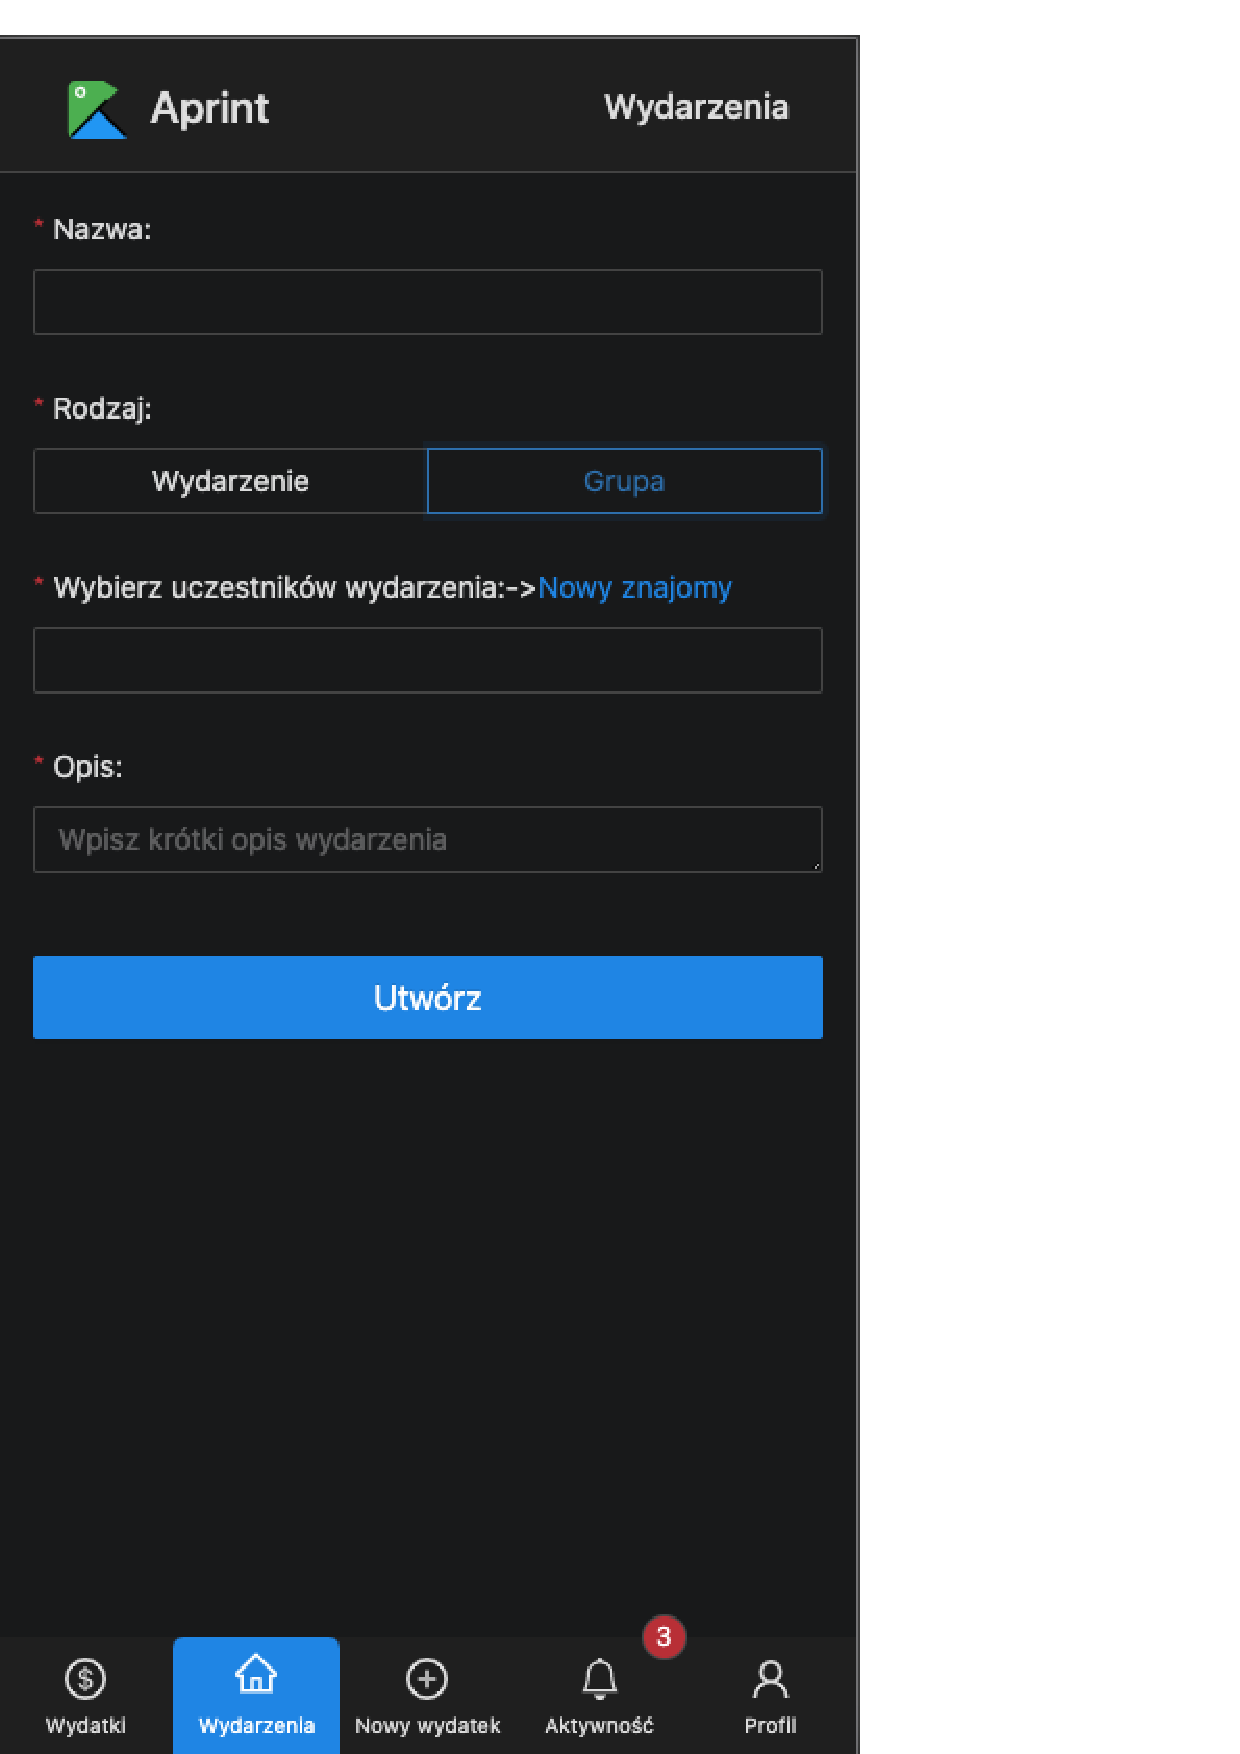
\includegraphics[width=0.45\textwidth]{presentation/event-group-form.png} }}%
    \caption{Formularz w trybie typu \emph{Grupa}}
\end{figure}

\clearpage
\subsection{Aktywność}
Panel aktywności wyświetla użytkownikowi wszystkie dostępne powiadomienia w formie listy. Po kliknięciu w elementy aplikacja przekieruje użytkownika do odpowiednich stron np. po kliknięciu w pierwszy element ukazany na rysunku ~\ref{fig:notificationList} zostaniemy przekierowywani do wydatku, do którego użytkownik został dołączony. Dodatkowo, gdy są na ekranie nowe powiadomienia, wyświetlają się przy nich czerwone kropki, aby zwrócić na nie uwagę użytkownika (przykład na rysunku ~\ref{fig:notificationListNew}). Każde powiadomienie może być usunięte przez użytkownika. Powiadomienia są posortowane w taki sposób, aby najnowsze pojawiały się na samej górze ekranu. Ekran spełnia wymaganie WF8.

\begin{figure}[h!]%
    \centering
    \subfloat[\centering Lista aktywności]{{\includegraphics[width=0.45\textwidth]{presentation/notification-list.png} \label{fig:notificationList} }}%
    \qquad
    \subfloat[\centering Lista aktywności z nowym powiadomieniem]{{\includegraphics[width=0.45\textwidth]{presentation/notification-list-new.png} \label{fig:notificationListNew}}}%
    \caption{Ekran listy powiadomień}%
\end{figure}

\clearpage
\subsection{Ekrany użytkownika}
\subsubsection{Ekran informacji o użytkowniku}
Na ekranie użytkownika są wyświetlone dane użytkownika tj. imię, numer konta, email. Z poziomu tego ekranu użytkownik może edytować te informacje oraz wylogować się z konta.

\begin{figure}[h!]%
    \centering
    \subfloat[\centering Informacje użytkownika]{{\includegraphics[width=0.45\textwidth]{presentation/user-profile.png} }}%
    \qquad
    \subfloat[\centering Edycja numeru konta]{{\includegraphics[width=0.45\textwidth]{presentation/user-change-number.png}}}%
    \caption{Ekran użytkownika}%
\end{figure}

\clearpage
\subsubsection{Ekran znajomych}
Na ekranie znajomych znajduje się lista wszystkich znajomych użytkownika oraz mechanizm dodawania nowych użytkowników. Dodatkowo z tego poziomu użytkownik może też usuwać innych użytkowników z listy swoich znajomych. Ekran spełnia wymaganie WF3.

\begin{figure}[h!]%
    \centering
    \subfloat[\centering Lista znajomych]{{\includegraphics[width=0.45\textwidth]{presentation/friend-list.png} }}%
    \qquad
    \subfloat[\centering Dialog dodawania nowych znajomych]{{\includegraphics[width=0.45\textwidth]{presentation/friend-add.png}}}%
    \caption{Ekran znajomych}%
\end{figure}

\clearpage
\subsubsection{Ekran innego użytkownika}
Użytkownik może też zobaczyć informacje o innym użytkowniku: jego email, imie oraz numer konta, na który może przelać pieniądze za płatność. Na tym ekranie dostępne są też informacje o balansie pieniężnym pomiędzy użytkownikami. Ekran spełnia wymaganie WF11.

\begin{figure}[h!]%
    \centering
    \subfloat[\centering Lista znajomych]{{\includegraphics[width=0.45\textwidth]{presentation/friend-view.png} }}%
\end{figure}
         % Wygodnie jest trzymać każdy rozdział w osobnym pliku.
                            % na nowe wersje, a cały tekst pracy pozostaje nienaruszony.

\newpage % Rozdziały zaczynamy od nowej strony
\section{Summatio}          % Można też pisać rozdziały w jednym pliku.
\lipsum[5-10]

%--------------------------------------------
% Literatura
%--------------------------------------------
\cleardoublepage % Zaczynamy od nieparzystej strony
\printbibliography

%--------------------------------------------
% Spisy (opcjonalne)
%--------------------------------------------
\newpage
\pagestyle{plain}

% Wykaz symboli i skrótów.
% Pamiętaj, żeby posortować symbole alfabetycznie
% we własnym zakresie. Ponieważ mało kto używa takiego wykazu,
% uznałem, że robienie automatycznie sortowanej listy
% na poziomie LaTeXa to za duży overkill.
% Makro \acronymlist generuje właściwy tytuł sekcji,
% w zależności od języka.
% Makro \acronym dodaje skrót/symbol do listy,
% zapewniając podstawowe formatowanie.
% //AB
\vspace{0.8cm}
\acronymlist
\acronym{EiTI}{Wydział Elektroniki i Technik Informacyjnych}
\acronym{PW}{Politechnika Warszawska}
\acronym{WEIRD}{ang. \emph{Western, Educated, Industrialized, Rich and Democratic}}

\listoffigurestoc     % Spis rysunków.
\vspace{1cm}          % vertical space
\listoftablestoc      % Spis tabel.
\vspace{1cm}          % vertical space
\listofappendicestoc  % Spis załączników

% Załączniki
\newpage
\appendix{Nazwa załącznika 1}
\lipsum[1-8]

\newpage
\appendix{Nazwa załącznika 2}
\lipsum[1-4]

% Używając powyższych spisów jako szablonu,
% możesz tu dodać swój własny wykaz bądź listę,
% np. spis algorytmów.

\end{document} % Dobranoc.
